\documentclass[a4paper, 11pt]{article}\usepackage[]{graphicx}\usepackage[]{color}
%% maxwidth is the original width if it is less than linewidth
%% otherwise use linewidth (to make sure the graphics do not exceed the margin)
\makeatletter
\def\maxwidth{ %
  \ifdim\Gin@nat@width>\linewidth
    \linewidth
  \else
    \Gin@nat@width
  \fi
}
\makeatother

\definecolor{fgcolor}{rgb}{0.345, 0.345, 0.345}
\newcommand{\hlnum}[1]{\textcolor[rgb]{0.686,0.059,0.569}{#1}}%
\newcommand{\hlstr}[1]{\textcolor[rgb]{0.192,0.494,0.8}{#1}}%
\newcommand{\hlcom}[1]{\textcolor[rgb]{0.678,0.584,0.686}{\textit{#1}}}%
\newcommand{\hlopt}[1]{\textcolor[rgb]{0,0,0}{#1}}%
\newcommand{\hlstd}[1]{\textcolor[rgb]{0.345,0.345,0.345}{#1}}%
\newcommand{\hlkwa}[1]{\textcolor[rgb]{0.161,0.373,0.58}{\textbf{#1}}}%
\newcommand{\hlkwb}[1]{\textcolor[rgb]{0.69,0.353,0.396}{#1}}%
\newcommand{\hlkwc}[1]{\textcolor[rgb]{0.333,0.667,0.333}{#1}}%
\newcommand{\hlkwd}[1]{\textcolor[rgb]{0.737,0.353,0.396}{\textbf{#1}}}%
\let\hlipl\hlkwb

\usepackage{framed}
\makeatletter
\newenvironment{kframe}{%
 \def\at@end@of@kframe{}%
 \ifinner\ifhmode%
  \def\at@end@of@kframe{\end{minipage}}%
  \begin{minipage}{\columnwidth}%
 \fi\fi%
 \def\FrameCommand##1{\hskip\@totalleftmargin \hskip-\fboxsep
 \colorbox{shadecolor}{##1}\hskip-\fboxsep
     % There is no \\@totalrightmargin, so:
     \hskip-\linewidth \hskip-\@totalleftmargin \hskip\columnwidth}%
 \MakeFramed {\advance\hsize-\width
   \@totalleftmargin\z@ \linewidth\hsize
   \@setminipage}}%
 {\par\unskip\endMakeFramed%
 \at@end@of@kframe}
\makeatother

\definecolor{shadecolor}{rgb}{.97, .97, .97}
\definecolor{messagecolor}{rgb}{0, 0, 0}
\definecolor{warningcolor}{rgb}{1, 0, 1}
\definecolor{errorcolor}{rgb}{1, 0, 0}
\newenvironment{knitrout}{}{} % an empty environment to be redefined in TeX

\usepackage{alltt}
\usepackage[colorlinks=true, urlcolor=blue,linkcolor=blue]{hyperref}
\usepackage{layout}
\usepackage[top=2cm, bottom=2cm, left=4cm, right=4cm]{geometry}

\title{Statistical Inference Assignement \\ ToothGrowth Datas Analysis}
\author{by Bruno Berrehuel}
\IfFileExists{upquote.sty}{\usepackage{upquote}}{}
\begin{document}
\maketitle

\section{Introduction}
The datas are about the length of odontoblast (cells responsible for tooth growth) for 60 pigs after an experimental threatment in vitamin C. Each animal received a dose of vitamin C, from 0.5 to 2 mg/day, by orange juice (OJ) or ascorbic acid (VC)\footnote{Source : \url{https://stat.ethz.ch/R-manual/R-devel/library/datasets/html/ToothGrowth.html}}. Each experiment deals with 10 pigs.

\noindent
I'll try to answer the two following questions :
\begin{enumerate}
    \item Q1 : is the vitamin C effective for tooth growth ?
    \item Q2 : what is the best delivery method between orange juice or ascorbic acid ?
\end{enumerate}

\section{Data exploratory}

First I'll take some informations about the means and the standard deviation of each dose, and plot the evolution of the tooth growth depending on the dose and the delivery method :
\begin{knitrout}\small
\definecolor{shadecolor}{rgb}{0.969, 0.969, 0.969}\color{fgcolor}\begin{kframe}
\begin{alltt}
\hlstd{ToothGrowth} \hlopt \hlkwd{group_by}\hlstd{(supp,dose)} \hlopt
    \hlkwd{summarise}\hlstd{(}\hlkwd{mean}\hlstd{(len),} \hlkwd{round}\hlstd{(}\hlkwd{sd}\hlstd{(len),}\hlnum{3}\hlstd{))}
\end{alltt}
\begin{verbatim}
## Source: local data frame [6 x 4]
## Groups: supp [?]
## 
##     supp  dose `mean(len)` `round(sd(len), 3)`
##   <fctr> <dbl>       <dbl>               <dbl>
## 1     OJ   0.5       13.23               4.460
## 2     OJ   1.0       22.70               3.911
## 3     OJ   2.0       26.06               2.655
## 4     VC   0.5        7.98               2.747
## 5     VC   1.0       16.77               2.515
## 6     VC   2.0       26.14               4.798
\end{verbatim}
\end{kframe}
\end{knitrout}
\begin{knitrout}
\definecolor{shadecolor}{rgb}{0.969, 0.969, 0.969}\color{fgcolor}
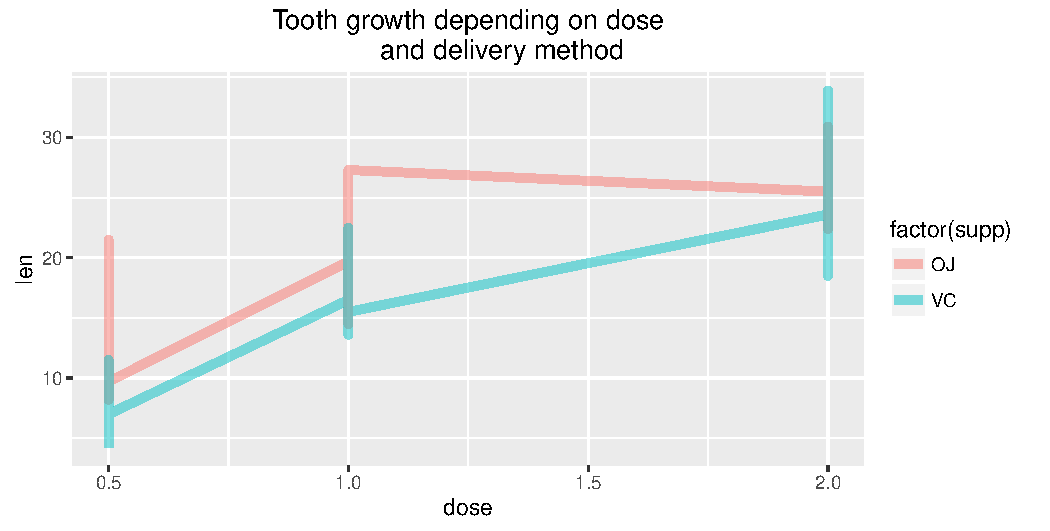
\includegraphics[width=\maxwidth]{figure/unnamed-chunk-2-1} 

\end{knitrout}

\noindent
It seems that : 
\begin{itemize}
    \item H1 : odontoblasts are taller with a bigger dose of vitamin C, no matter of the delivery method.
    \item H2 : orange juice (OJ) has better results than ascorbic acid (VC).
\end{itemize}

\section{Probability tests}

I define some variables form the ToothGrowth datasets, in order to compare with the R function \textbf{t.test} :
\begin{itemize}
    \item H1 : the mean of odontoblasts length at 0.5 mg/day dose with the mean at 2 mg/day
    \item H2 : the means of odontoblasts length for the 2 delivery method ar each vitamin C dose.
\end{itemize}
\subsection{Tests for H1 hypothesis}
First filter the ToothGrowth dataset depending on dose of vitamin C, for both of the delivery method, then do t.test to confirm that the mean at 2 mg/day is more important than the mean at 0.5 mg/day.

\begin{knitrout}\small
\definecolor{shadecolor}{rgb}{0.969, 0.969, 0.969}\color{fgcolor}\begin{kframe}
\begin{alltt}
\hlstd{vita05} \hlkwb{<-} \hlstd{ToothGrowth} \hlopt \hlkwd{filter}\hlstd{(dose}\hlopt{==}\hlnum{0.5}\hlstd{)}
\hlstd{vita2} \hlkwb{<-} \hlstd{ToothGrowth} \hlopt \hlkwd{filter}\hlstd{(dose}\hlopt{==}\hlnum{2}\hlstd{)}
\hlkwd{t.test}\hlstd{(vita2}\hlopt{$}\hlstd{len}\hlopt{-}\hlstd{vita05}\hlopt{$}\hlstd{len,} \hlkwc{alternative}\hlstd{=}\hlstr{"greater"}\hlstd{)}
\end{alltt}
\begin{verbatim}
## 
## 	One Sample t-test
## 
## data:  vita2$len - vita05$len
## t = 11.291, df = 19, p-value = 3.595e-10
## alternative hypothesis: true mean is greater than 0
## 95 percent confidence interval:
##  13.12216      Inf
## sample estimates:
## mean of x 
##    15.495
\end{verbatim}
\end{kframe}
\end{knitrout}

\subsection{Tests for H2 hypothesis}
First filter the ToothGrowth dataset depending on dose of vitamin C and delivery method, then compare them with the t.test function.
\begin{knitrout}\small
\definecolor{shadecolor}{rgb}{0.969, 0.969, 0.969}\color{fgcolor}\begin{kframe}
\begin{alltt}
\hlstd{indice} \hlkwb{<-} \hlkwd{c}\hlstd{(}\hlnum{0.5}\hlstd{,}\hlnum{1}\hlstd{,}\hlnum{2}\hlstd{)}
\hlstd{OJ} \hlkwb{<-} \hlkwd{lapply}\hlstd{(indice,} \hlkwa{function}\hlstd{(}\hlkwc{i}\hlstd{) \{ToothGrowth} \hlopt \hlkwd{filter}\hlstd{(supp}\hlopt{==}\hlstr{"OJ"}\hlstd{)} \hlopt
             \hlkwd{filter}\hlstd{(dose}\hlopt{==}\hlstd{i)\})}
\hlstd{VC} \hlkwb{<-} \hlkwd{lapply}\hlstd{(indice,} \hlkwa{function}\hlstd{(}\hlkwc{i}\hlstd{) \{ToothGrowth} \hlopt \hlkwd{filter}\hlstd{(supp}\hlopt{==}\hlstr{"VC"}\hlstd{)} \hlopt
             \hlkwd{filter}\hlstd{(dose}\hlopt{==}\hlstd{i)\})}
\hlkwd{t.test}\hlstd{(OJ[[}\hlnum{1}\hlstd{]]}\hlopt{$}\hlstd{len}\hlopt{-}\hlstd{VC[[}\hlnum{1}\hlstd{]]}\hlopt{$}\hlstd{len,} \hlkwc{alternative}\hlstd{=}\hlstr{"greater"}\hlstd{)}
\end{alltt}
\begin{verbatim}
## 
## 	One Sample t-test
## 
## data:  OJ[[1]]$len - VC[[1]]$len
## t = 2.9791, df = 9, p-value = 0.007736
## alternative hypothesis: true mean is greater than 0
## 95 percent confidence interval:
##  2.019552      Inf
## sample estimates:
## mean of x 
##      5.25
\end{verbatim}
\begin{alltt}
\hlkwd{t.test}\hlstd{(OJ[[}\hlnum{2}\hlstd{]]}\hlopt{$}\hlstd{len}\hlopt{-}\hlstd{VC[[}\hlnum{2}\hlstd{]]}\hlopt{$}\hlstd{len,} \hlkwc{alternative}\hlstd{=}\hlstr{"greater"}\hlstd{)}
\end{alltt}
\begin{verbatim}
## 
## 	One Sample t-test
## 
## data:  OJ[[2]]$len - VC[[2]]$len
## t = 3.3721, df = 9, p-value = 0.004115
## alternative hypothesis: true mean is greater than 0
## 95 percent confidence interval:
##  2.706401      Inf
## sample estimates:
## mean of x 
##      5.93
\end{verbatim}
\begin{alltt}
\hlkwd{t.test}\hlstd{(OJ[[}\hlnum{3}\hlstd{]]}\hlopt{$}\hlstd{len}\hlopt{-}\hlstd{VC[[}\hlnum{3}\hlstd{]]}\hlopt{$}\hlstd{len)}
\end{alltt}
\begin{verbatim}
## 
## 	One Sample t-test
## 
## data:  OJ[[3]]$len - VC[[3]]$len
## t = -0.042592, df = 9, p-value = 0.967
## alternative hypothesis: true mean is not equal to 0
## 95 percent confidence interval:
##  -4.328976  4.168976
## sample estimates:
## mean of x 
##     -0.08
\end{verbatim}
\end{kframe}
\end{knitrout}
\noindent
We have the following results :
\begin{itemize}
    \item we can reject  $\mu_{OJ05} = \mu_{VC05}$ and accept  $\mu_{OJ05} > \mu_{VC05}$
    \item we can reject  $\mu_{OJ1} = \mu_{VC1}$ and accept  $\mu_{OJ1} > \mu_{VC1}$
    \item we failed to reject  $\mu_{OJ2} = \mu_{VC2}$
\end{itemize}

\section{Conclusions}
\subsection{Is the vitamin C effective for tooth growth ?}
As the t.test shows that the real mean of the 2 mg/day tooth growth is greater than the 0.5 mg/day tooth growth, the vitamin C threatment is effective for the pigs.
\subsection{What is the best delivery method ?}
The t.tests show that :
\begin{itemize}
    \item the orange juice delivery method is more effective than the ascorbic acid method for small doses, as the real tooth growth means are greater for orange juice for 0.5 and 1 mg/day doses.
    \item the methods are equivalent for the dose 2 mg/day, as we failed to reject the null hypothesis that the means are equal.
\end{itemize}
\fbox{
    \parbox[c][1.5\height]{\textwidth}{
        \textbf{I recommend the delivery of vitamin C, by orange juice, for the tooth growth of the guinea pigs.}}}
\end{document}
